\subsection{Creating Custom Analysis Routines and Calculating Rate Constants}

\subsubsection{Introduction}

In this tutorial, we will go over how to create custom analysis routines using the \verb|westpa.analysis| Python API and how to calculate rate constants using the Rate from Event Durations (RED) analysis scheme, which enables rate-constant estimates from transient, pre- steady-state data and therefore shares the same motivation as the haMSM analysis scheme \citep{copperman_accelerated_2020,russo_westpa_2022} used in the above \textbf{Advanced Tutorial 3.3}.
For the creation of custom analysis routines, we will focus on the membrane permeability simulations completed in \textbf{Advanced Tutorial 3.2}.
For the calculation of rate constants, we will focus on previously published protein-protein binding simulations involving the barnase/barstar system \citep{saglam_proteinprotein_2019}.   

\textbf{Learning objectives.} Specific learning objectives for this tutorial include:
\begin{enumerate}
    \item How to access simulation data in a \verb|west.h5| file using the high-level \verb|Run| interface of the \verb|westpa.analysis| Python API and how to retrieve trajectory data using the \verb|BasicMDTrajectory| and \verb|HDF5MDTrajectory| readers;
    \item How to access steady-state populations and fluxes from the \verb|assign.h5| and \verb|direct.h5| data files, convert fluxes to rate constants, and plot the rate constants using an appropriate averaging scheme;
    \item How to apply the RED analysis scheme to estimate rate constants from shorter trajectories.
\end{enumerate}

\subsubsection{Prerequisites}
In addition to completing the Basic and Intermediate WESTPA tutorials \citep{bogetti_suite_2019}, a prerequisite to this tutorial is completion of the above \textbf{Advanced Tutorials 3.1 and 3.2}.

\textbf{Computational requirements.} Users should have access to at least 1 CPU core for running the analysis tools.
For larger datasets, one may want to parallelize some of the tools (especially \verb|w_direct|).
The size of a dataset is mainly determined by the number of iterations. For a dataset of greater than 1000 iterations, it may be best to use at least 4 CPU cores at a time.

\subsubsection{Creating custom analysis routines}
For this part of the tutorial, we will create custom analysis routines using the \verb|westpa.analysis| API for the membrane permeability simulations completed in \textbf{Advanced Tutorial 3.2}. 

The main abstraction of the \verb|westpa.analysis| API is the \verb|Run| class, which provides a read-only view of the data in the main WESTPA output file (\verb|west.h5|).
We will start by opening the \verb|west.h5| file from the permeability run.
We assume that the current working directory is the simulation root directory you are interested in analyzing, though the resulting \verb|west.h5| file from \textbf{Advanced Tutorial 3.2} is linked to the main directory of this tutorial for convenience.
Open a Python interpreter and run the following commands.

\begin{verbatim}
  >>> from westpa.analysis import Run
  >>> run = Run.open(‘west.h5’)
  >>> run
    
<WESTPA Run with 500 iterations at 0x7fcaf8f0d5b0>
\end{verbatim}

We now have convenient access to a wealth of information about the permeability simulation, including all trajectory segments at each WE iteration and any data associated with those segments, including values of the progress coordinate and other auxiliary data.
Iterating over a run yields a sequence of \verb|Iteration| objects, each of which is a collection of \verb|Walker| objects.
For example, the following loop iterates over all trajectory walkers in a run, but does nothing with each trajectory walker:

\begin{verbatim}
  >>> for iteration in run:
  ...     for walker in iteration:
  ...         pass
\end{verbatim}

We can access a walker by providing its (1-based) iteration number and (0-based) segment ID:

\begin{verbatim}
  >>> walker = run.iteration(10).walker(4)
  >>> walker
Walker(4, Iteration(10, <WESTPA Run
    with 500 iterations at 0x7fcaf8f0d5b0>))
\end{verbatim}

To access the progress coordinates of a certain trajectory walker, we use the \verb|pcoords| attribute:

\begin{verbatim}
  >>> pcoords = walker.pcoords
\end{verbatim}

Other properties available through this Python API include the weight, parent and children of a trajectory walker.
We can access auxiliary data by looking up the dataset of interest in the \verb|auxiliary_data| dictionary attribute (note that the following auxiliary dataset is not actually present, and the command is provided as an example):

\begin{verbatim}
  >>> auxdata = walker.auxiliary_data[‘test_data’]
\end{verbatim}

We can also view a list of all recycled (successful) trajectory walkers and choose one walker to trace its pathway through the membrane:

\begin{verbatim}
  >>> walkers = run.recycled_walkers
  >>> walker = max(walkers, 
  ...    key=lambda walker: walker.weight)
\end{verbatim}

The history of a trajectory walker can be traced by using the \verb|trace()| method, which returns a \verb|Trace| object:

\begin{verbatim}
  >>> trace = walker.trace()
\end{verbatim}

Using the WE iteration and IDs of the trajectory segments obtained from this trace, we can plot the data of our traced trajectory to see how that property is changing.
Remember that the \verb|test_data| auxiliary dataset does not actually exist, but can be replaced with an auxiliary dataset of your choice.

\begin{verbatim}
  >>> xs = [walker.iteration.number 
  ...       for walker in trace]
  >>> ys = [walker.auxiliary_data[‘test_data’] 
  ...       for walker in trace]
  >>> import matplotlib.pyplot as plt
  >>> plt.plot(xs, ys)
\end{verbatim}

One goal of the \verb|westpa.analysis| API is to simplify the retrieval of trajectory coordinates.
Two built-in readers are provided for retrieving MD trajectory coordinates: (1) \verb|BasicMDTrajectory|, which handles trajectory files outputted by the dynamics engine; or (2) \verb|HDF5MDTrajectory|, which handles trajectories stored using the new HDF5 framework, as is done in the above \textbf{Tutorial 3.1 and 3.2}.
For users requiring greater flexibility, custom trajectory readers can be implemented using the more general \verb|Trajectory| class.
Here we provide a brief overview of both the \verb|BasicMDTrajectory| and the \verb|HDF5MDTrajectory| readers.
The following is included only as an example, since the trajectory files required are not provided.
MD trajectories stored in the traditional manner may be retrieved using the \verb|BasicMDTrajectory| reader with its default settings:

\begin{verbatim}
    >>> from westpa.analysis import BasicMDTrajectory
    >>> trajectory = BasicMDTrajectory()
\end{verbatim}

Here, \verb|trajectory| is a callable object that takes either a \verb|walker()| or a \verb|trace()| object as input and returns an \verb|mdtraj.Trajectory()| object ({\url{https://mdtraj.org/1.9.5/api/generated/mdtraj.Trajectory.html}}).
To retrieve the trajectory of the trace obtained above, then save the coordinates to a DCD file (e.g., for visualization using the VMD program), we can run the following:

\begin{verbatim}
    >>> traj = trajectory(trace)
    >>> traj.save(‘trace-coords.dcd’)
\end{verbatim}

Note that in the code above, we have relied on the fact that the \verb|traj_segs/| directory of interest is contained in the current working directory.
In the general case, the name of the simulation root directory may be provided to the trajectory reader via the optional \verb|sim_root| parameter.
Minor variations of the "basic" trajectory storage protocol (e.g., use of different file formats) can be handled by changing the parameters of the \verb|BasicMDTrajectory| reader: 

\begin{verbatim}
    >>> trajectory = BasicMDTrajectory(
        traj_ext='.nc', state_ext='.ncrst', top=None)
\end{verbatim}

However, suppose that instead of storing the coordinate and topology data for trajectory segments in separate files (\verb|seg.dcd| and \verb|bstate.pdb|), we store them together in an HDF5 trajectory file (such as \verb|iter_XXXXXX.h5|) using the new HDF5 restarting framework available in WESTPA 2.0. This change can be accommodated by using the \verb|HDF5MDTrajectory| reader:

\begin{verbatim}
    >>> trajectory = HDF5MDTrajectory()
\end{verbatim}

The examples above highlight the flexibility and convenience provided by the \verb|westpa.analysis| package and provide the building blocks available to a user wanting to explore the \verb|west.h5| file and create custom analysis routines using data in the \verb|west.h5| file.

\subsubsection{Calculating rate constants using the original WE scheme}

For the two remaining sections of this tutorial, we will focus on applying the RED analysis scheme \citep{degrave_red_2021} to calculate the association rate constant from previously published protein-protein binding simulations involving the barnase/barstar system \citep{saglam_proteinprotein_2019}.
The RED scheme involves three steps:

\textbf{1. Calculate State Populations and the Flux into the Target State.} The target state can be defined using either the WE progress coordinate or auxiliary coordinates.
The analysis bins and state definitions are placed in the analysis section of the \verb|west.cfg| file.

\begin{verbatim}
  west:
    analysis:
      kinetics:
           evolution: cumulative
         analysis_schemes:                  
           OVERALL:
             enabled: True
             bins:
               - type: RectilinearBinMapper
                 boundaries:
                   - [0, 3.5, 'inf']  
                   - [0, 3, 15, 'inf']
             states:
               - label: unbound
                 coords:
                   - [0.5, 50.0]
                   - [50.0, 50.0]
               - label: bound
                 coords: 
                   - [0.5, 0.5]
\end{verbatim}

To calculate the flux into a state defined by the progress coordinate, we can use the \verb|w_ipa| program. Flux calculation with \verb|w_ipa| involves two steps: (1) assigning trajectory segments to states using the \verb|w_assign| command-line tool, and (2) calculating the probability flux between each pair of defined states using the \verb|w_direct| command-line tool.
Given the large size of the barnase-barstar simulation HDF5 file, we have provided the resulting \verb|assign.h5| and \verb|direct.h5| files for the remainder of the tutorial.
To use \verb|w_ipa| for flux analysis, one would run the following at the command line:  

\begin{verbatim}
    $ w_ipa -ao
\end{verbatim}

This command will analyze the \verb|pcoord| data from \verb|west.h5| using the scheme for bins and states defined in \verb|west.cfg| and not drop the user into an IPython environment (to make use of that functionality, remove the \verb|-ao| options from the above command).
The resulting \verb|assign.h5| and \verb|direct.h5| files, the latter containing the fluxes, will be outputted to a newly created directory that is named for the relevant scheme (in this case that will be in \verb|./ANALYSIS/OVERALL/|.
The \verb|evolution:cumulative| option (which is the default option) ensures that all evolution datasets are calculated with a rolling average, a requirement for using the RED scheme (see below). 

To calculate the flux into a state defined by auxiliary coordinates, we still use the scheme for bins and states defined in the \verb|west.cfg| file.
However, instead of using the \verb|w_ipa| program, we use the command-line tools, \verb|w_assign| and \verb|w_direct|.
Before using these tools, we need to copy \verb|module.py| to your current directory first (by default, \verb|module.py| is located in the \verb|./scripts/| directory).
Then, we can assign trajectory segments to specified states using the \verb|w_assign| tool:

\begin{verbatim}
  $ w_assign --config-from-file --scheme OVERALL 
    --construct-dataset module.load_auxdata --serial
\end{verbatim}

The \verb|--config-from-file| option tells the program to read analysis parameters from the \verb|west.cfg| file’s analysis section and the \verb|--scheme| option specifies the relevant scheme for bins and states.
The \verb|--construct-dataset| option provides a function to \verb|w_assign| for loading in the auxiliary data which is located in the file \verb|module.py|.
The \verb|--serial| option tells \verb|w_assign| to run the assignment in serial mode.
Running \verb|w_assign| will generate an \verb|ANALYSIS/| directory and place an \verb|assign.h5| file in a scheme-specific folder there.
Next, we apply the \verb|w_direct| tool to the \verb|assign.h5| file.

\begin{verbatim}
  $ w_direct all -a ./ANALYSIS/OVERALL/assign.h5
\end{verbatim}

This command will generate a \verb|direct.h5| file in the same directory where we ran the \verb|w_direct| command.
Move this file to the \verb|analysis/| folder that was generated by \verb|w_assign| and proceed with the analysis.
Note that the above is not part of the following tutorial and is only included to provide an example to users of how to perform an analysis on auxiliary data.

\textbf{2. Correct the Fluxes using the RED Scheme.} To correct the calculated fluxes using the RED scheme, we apply the \verb|w_red| command-line tool, which will read in the \verb|rate_evolution| and durations datasets in your \verb|direct.h5| file and calculates a correction factor for the flux value at each iteration.
To use this tool, add the following to the analysis section of your \verb|west.cfg| file:
\begin{verbatim}
  red:
    scheme: OVERALL
    istate_label: unbound
    fstate_label: bound
    nstiter: 21
    nstrep: 1
\end{verbatim}

\noindent For the scheme option, specify  the desired scheme for bins and states to use from your \verb|west.cfg| analysis section and for the \verb|istate_label| and \verb|fstate_label| options, specify the initial and target states, respectively.
The \verb|nstiter| parameter is the number of frames per WE iteration that were saved during the WESTPA simulation and \verb|nstrep| is the frequency of outputting progress of the RED calculation. After setting all parameters, run the \verb|w_red| tool from the command line:

\begin{verbatim}
  $ w_red
\end{verbatim}

\noindent A new dataset containing the corrected fluxes, named \verb|red_flux_evolution|, will be added to your \verb|direct.h5| file.
If that dataset already exists, the \verb|w_red| tool will ask if you want to overwrite the existing dataset.

The new \verb|red_flux_evolution| dataset is created by adjusting the \verb|rate_evolution| dataset by the correction factor determined by the RED scheme.
The \verb|rate_evolution| dataset, in turn, is composed of the relevant \verb|conditional_flux_evolution| dataset (from \verb|direct.h5|) normalized by the steady state populations from \verb|labeled_populations| (from \verb|assign.h5|).
Therefore, when using the RED scheme (or the original \verb|rate_evolution| dataset), no explicit normalization of the fluxes by the steady state populations is necessary.

\textbf{3. Convert the Flux to a Rate Constant.} The fluxes that we just calculated are already rate constants in units of inverse $\tau$ (the resampling interval used for your WE simulation). 

For a unimolecular process, the final units of the rate constant should be inverse time (e.g., s\textsuperscript{-1}) and can be obtained by converting from units of per $\tau$ for the extracted flux array to the desired time unit.
Note that the $\tau$ value needs to be provided by the user and is not currently recorded in the \verb|west.h5| file.

For a bimolecular process, which is the case for our \verb|OVERALL| scheme, the rate constant should be in units of inverse time and inverse concentration (e.g., M\textsuperscript{-1}s\textsuperscript{-1}) and can be obtained by first converting to the desired time unit, as done for unimolecular processes, and dividing the resulting flux values by the effective concentration of the solutes involved in the bimolecular process given the volume of the simulation box.
In the case of our barnase-barstar system, the $\tau$ value was 20 ps and the effective concentration for the barstar ligand was 1.7 mM.
We will therefore divide all of the \verb|conditional_flux| values by 20 $\times$ 10\textsuperscript{-12} s and 0.0017 M to obtain per iteration rate constants in units of M\textsuperscript{-1}s\textsuperscript{-1}.

\subsubsection{Monitoring Convergence of the Rate Constant}  

To monitor the convergence of the rate-constant estimate, we can plot the time-evolution of the rate constant using both the original and RED schemes and assess how close our original estimate is to the RED estimate.
If the two schemes are converging to the same value, that can be one indication that the simulation has begun to converge.

To obtain the rate constant using the original scheme \citep{huber_weighted-ensemble_1996}, simply convert the \verb|rate_evolution| dataset to the appropriate units as discussed above.
The time-evolution of this rate-constant estimate can then be compared with the RED-scheme estimate to assess convergence of the simulation to a steady state (\textbf{Figure 8A}).

\begin{figure}[ht]
\centering
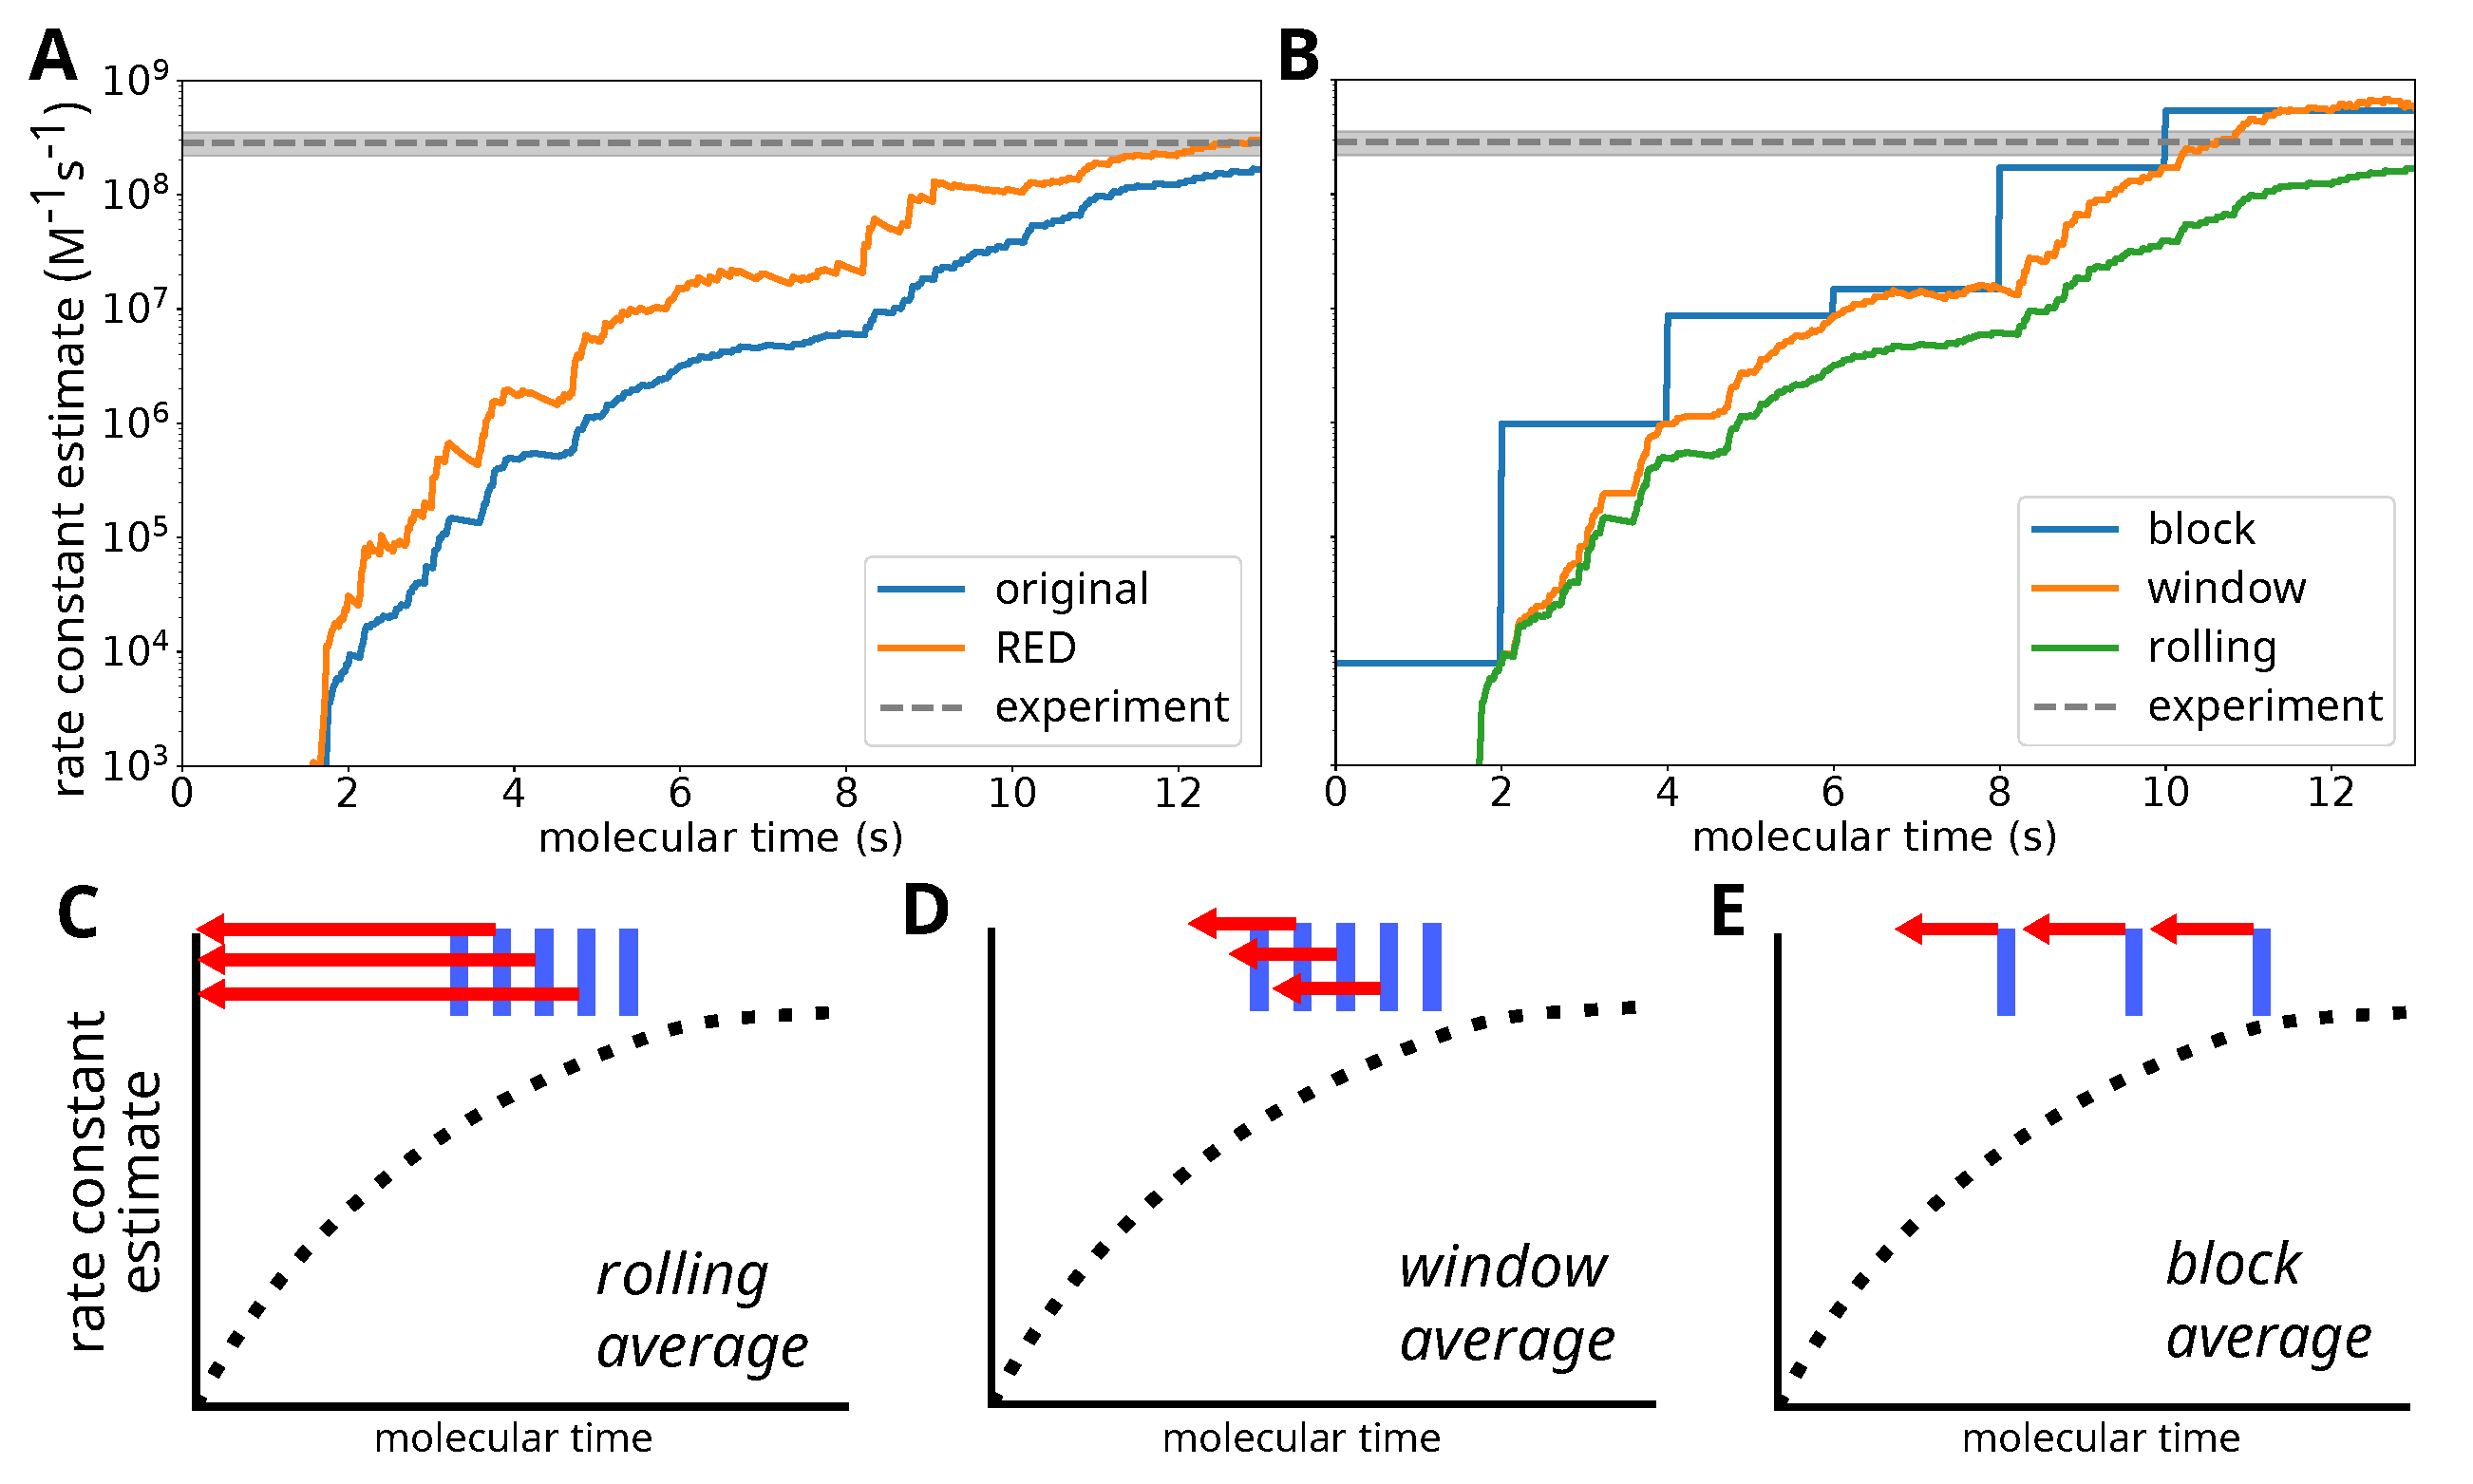
\includegraphics[width=\columnwidth]{figures/Figure8_analysis.pdf}
\caption{A) A comparison of the RED and original schemes for estimating the rate constant for protein-protein association involving the barnase/barstar system from previously published WE simulations \citep{saglam_proteinprotein_2019}.
In this case, the simulation has not converged to a steady state, as indicated by different rate-constant estimates using the original and RED schemes.
B) A comparison of different averaging schemes using the same dataset.
While the RED scheme is, in principle, only compatible with rolling averages, the use of block and window averaging can still be informative for monitoring convergence of the simulation.
C-E) Schematic illustrations of rolling, window, and block averaging schemes, indicating points where averages are calculated (blue) and the extent of data used for the averages (red).}
\end{figure}

\textbf{A note on averaging schemes.} 
There are three main types of averaging schemes that can be used to monitor convergence when plotting the rate constant evolution using the original scheme.
It may be useful to plot different schemes depending on the behavior of your specific system.
A few examples are shown here with instructions on how to generate the plots.

The first averaging scheme is the default which is a rolling average (\textbf{Figure 8B}), which can be achieved by specifying \verb|evolution: cumulative| in the analysis section of \verb|west.cfg| and setting \verb|step_iter: 1|.
This method of visualizing the rate constant evolution offers the smoothest curve and is recommended as the most stringent way of assessing convergence, as it incorporates information from the entire simulation.
A rolling average is also implicitly incorporated into the RED scheme, which by design never excludes data from the start of a simulation.
When analyzing rate constant estimates generated by the RED scheme, specify \verb|evolution: cumulative| to ensure that only the implicit rolling average is performed.

The second averaging scheme is a window average, which can be achieved in \verb|w_ipa| by specifying \verb|evolution: cumulative| and \verb|step_iter: 10|, or whatever your desired averaging window is.
A recommended starting averaging window size is 10\% of the length of your simulation, but the most robust would be the lag time of your simulation as determined from an autocorrelation of the flux plot.
A windowed average is not as smooth as the rolling average but can give a better indication of convergence at different stages of your simulation relative to other stages.

The third and final averaging scheme is a block average.
This will require setting \verb|evolution: blocked| and \verb|step_iter: 10|.
The rationale behind choosing the block size here is the same as the window size discussed above.
The block average will appear like a step function where each block an average of the preceding block is plotted.
This method of plotting is the least smooth, but can be best for obtaining a final value of the rate constant that is not influenced by earlier, lower values.

\subsubsection{Conclusion}

Among the upgrades introduced in the WESTPA 2.0 software package are ones that enable the creation and execution of more streamlined analysis of simulations and more efficient estimation of rate constants.
The \verb|westpa.analysis| subpackage can be utilized to more carefully inspect WESTPA trajectory data and to create custom analysis routines.
The RED analysis scheme for correcting rate constants based on the “ramp-up” time in the fluxes is implemented in the \verb|w_red| command-line tool.
The files contained in this tutorial for utilizing the RED scheme are intended to provide useful starting points for analyzing the kinetics of WESTPA simulations.